\documentclass[a4paper]{article}
% \documentclass[a4paper]{book}

% Imports
\usepackage[utf8]{inputenc}
\usepackage[ngerman]{babel}
\usepackage[T1]{fontenc}
\usepackage{fancyhdr}
\usepackage{caption}
\usepackage{float}
\usepackage{subcaption}
\usepackage{epigraph}
\usepackage{subfiles}
\usepackage[acronym]{glossaries}
\usepackage{graphicx}
\usepackage[style=apa]{biblatex}
\usepackage{pdfpages}
\usepackage{attachfile2}
\usepackage{tabularx}
\usepackage{hyperref}

\bibliography{./Bibliography}

% Generate the glossary
\makeglossaries

% Title page
\title{Open Source Software \\
    \noindent\rule[0.25ex]{\linewidth}{0.5pt}
    \large Wie nehmen Endanwender Open Source Software wahr?
}

\author{
  Blechschmidt, Til\\
  \texttt{til@blechschmidt.de}\\
  Nordakademie, Elmshorn
  \and
  Peeters, Noah\\
  \texttt{noah.peeters@icloud.com}\\
  Nordakademie, Elmshorn
}

% Numbering
\setcounter{secnumdepth}{3}
\setcounter{tocdepth}{2}

% Quote styling
\setlength\epigraphwidth{.8\textwidth}
\setlength\epigraphrule{0pt}

% Glossery
% \newglossaryentry{oss}{name=OSS, description={Open Source Software}}
\newacronym{oss}{OSS}{Open Source Software}


\begin{document}
    % Title page
    \thispagestyle{fancy}
    \maketitle

    % Abstract
    \begin{abstract}
         \gls{oss} wird in vielen Bereichen eingesetzt. In dieser Arbeit wird analysiert, wie Endanwender \gls{oss} wahrnehmen.
    \end{abstract}
    \newpage

    % TOC
    \tableofcontents
    \listoffigures
    \listoftables
    \clearpage

    % --- Content ---
    
                    
    \section{Fragestellung}
        In der Arbeit soll die Frage, inwiefern Endanwender Open Source Software wahrnehmen, untersucht werden. Dabei soll nicht nur die \emph{direkte} Verwendung von Open Source Software, wie es zum Beispiel bei LibreOffice der Fall ist, eine Rolle spielen, sondern auch die \emph{indirekte} Nutzung als Komponente kommerzieller Lösungen wie Chromium bzw. WebKit als Basis von Google Chrome\footcite{is:open:source:right:for:you} aber auch als Werkzeug wie Linux als Betriebssystem für Server\footcite{report:BaselineScenario}.
		
		Es wird erwartet, dass viele Nutzer unbewusst und indirekt mit Open Source Software in Kontakt stehen, sie diese also als Teil größerer, kommerzieller Closed Source Software nutzen, sich dessen aber nicht bewusst sind. Außerdem ist zu erwarten, dass nur ein kleiner Teil der Anwender direkt mit Open Source Software interagiert\footcite{oss:lotus-to-linux}.
		
		Um zuverlässige Daten zu erhalten, die die aktuelle Wahrnehmung der Endanwender widerspiegeln, wird eine Umfrage durchgeführt. Für die Sicherstellung der Repräsentativität der Umfrage werden mindestens 80 Antworten erwartet.
		Die Umfrage wird quantitativ mit geschlossenen Fragen gestaltet, um den Aufwand für die Befragten zu minimieren und damit die Teilnehmerrate und Datenmenge zu maximieren. % TODO: Cite
		
		\subsection{Definitionen} % TODO: Achtung Reihenfolge Definitionen/Fragestellung
            \subsubsection{Open Source Software}
                \begin{quote} 
                    \centering 
                    Software wird als Open Source bezeichnet, wenn ihr Quelltext frei zugänglich ist. Sie kann in kommerzieller Software eingesetzt werden, ihre Nutzung muss allerdings nicht kostenfrei sein. 
                \end{quote}
                
            \subsubsection{Nutzung von Open Source Software}
                Die Nutzung von Open Source Software durch Endanwender kann in zwei Arten unterschieden werden.
                
                \paragraph{Direkte Nutzung}
                    Zum einen gibt es die direkte Nutzung, bei der der Nutzer eine Software verwendet, die Open Source ist, also dessen Source Code frei zugänglich ist.
                    
                    Beispiele für Direkte Nutzung:
                    \begin{itemize}
                        \item Wikipedia\footnote{Wikipedia ist eine Konfiguration von Wikimedia, dessen Source Code frei zugänglich ist (\fullcite{wikimedia:download}).}
                        \item Thunderbird\footnote{\fullcite{thunderbird:faq}}
                        \item ... % TODO: mehr Beispiele
                    \end{itemize}
                    
                \paragraph{Indirekte Nutzung}
                    Zum anderen gibt es die indirekte Nutzung. Hier verwendet der Nutzer Software, dessen Source Code nicht frei zugänglich ist, deren Funktionalität aber entscheidend von \gls{oss} Komponenten abhängt. Ohne diese Komponenten wäre die Funktionalität stark eingeschränkt. Hierbei werden folgende Komponenten \textbf{nicht} berücksichtigt:
                    
                    \begin{itemize}
                        \item Entwicklerwerkzeuge wie Compiler
                        \item Datenbanken wie MySQL
                        \item Betriebssysteme wie Linux 
                        \item ... % TODO: gibt es mehr? Apache Web server?
                    \end{itemize}
                    Der Grund dafür liegt in der Verbreitung dieser Komponenten. % TODO: bessere Erklärung
                    
                    Beispiele für Indirekte Nutzung:
                    \begin{itemize}
                        \item Google Chrome\footnote{\fullcite{chromium:homepage}}
                        \item macOS\footnote{\fullcite{apple:oss}}
                        \item ... % TODO: mehr Beispiele
                    \end{itemize}

            
        
    \section{Design und Durchführung}
		Zweck der Befragung ist es, einen repräsentativen Überblick über die Wahrnehmung von Open Source Software des Endanwenders zu erhalten. Dabei soll Aufschluss über die Verteilung von indirekter sowie direkter Nutzung gegeben werden und in dem Zusammenhang analysiert werden, warum sich Anwender für Open Source Software entscheiden. Außerdem soll evaluiert werden, welche Gründe die Nutzer für und gegen die Nutzung von Open Source Software sehen.
	
		\subsection{Design}
		  \subsubsection{Aufbau}
    			Die Erhebung ist in vier Teile gegliedert, die im Folgenden näher erläutert sind: 
    		   
    			\paragraph{Bewusste Nutzung}
    				Um die, dem Anwender bewusste, Nutzung von Open Source Software zu erheben, beginnt die Umfrage mit diesem Abschnitt.\\
    				Zunächst wird ermittelt, ob die Nutzer wissen, was Open Source Software ist. Um im weiteren Verlauf der Umfrage sinnvolle Antworten zu erhalten, wird anschließend die Definition von Software sowie quelloffener Software erklärt.\\
    				Nun werden Fragen zum Nutzungsverhalten von solcher Software gestellt ohne dabei Beispiele zu nennen, um Beeinflussung zu vermeiden.
    			
    			\paragraph{Unbewusste Nutzung}
    				Im zweiten Abschnitt werden konkrete Beispiele für Open Source Software genannt, um die Nutzer darauf aufmerksam zu machen, wo Open Source Komponenten und Softwares überall eingesetzt werden, ohne dass es ihnen klar ist.\\
    				Außerdem soll geklärt werden, warum es Differenzen, wenn vorhanden, zwischen bewusster und unbewusster Nutzung gibt.
    			
    			\paragraph{Gründe für und gegen Open Source Software}
    				Im dritten Abschnitt werden Fragen bezüglich der Nutzungs- und Hinderungsgründe von Open Source Software gestellt. Dazu wird gefragt, warum oder warum nicht Endnutzer oder Unternehmen Open Source Software einsetzten. Die möglichen Antworten werden aus der Schweizer Studie zum Thema Open Source\footcite{oss:studie} genommen, um die Wahrnehmung mit der realen Nutzung vergleichbar zu machen.
    			
    			\paragraph{Demographische Differenzen}
    				Zur Analyse von Differenzen innerhalb der Bevölkerungen enthält die Umfrage Fragen zur aktuellen Tätigkeit\footnote{Schüler, Student, Arbeitnehmer, etc.} sowie zur Selbsteinschätzung der Computerkenntnisse.
				
			\subsubsection{Designentscheidungen}
			 \begin{itemize}
			     \item Es wurde überwiegend auf Freifelder verzichtet, um die Auswertung zu vereinfachen. Deshalb wurde bei dem eingesetzten Freifeld ein einheitliches Format gefordert.
				\item Bei Skalen wurde darauf geachtet eine gerade Anzahl an Optionen anzubieten, um den Nutzer nicht die Möglichkeit zu bieten neutral zu antworten.
				\item Die Texte sollen möglichst allgemeinverständlich geschrieben sein, um auch Nutzern ohne technischen Hintergrund die Teilnahme an der Umfrage zu ermöglichen.
			 \end{itemize}
			     
		\subsection{Durchführung}
            \subsubsection{Verbreitung}
                Um die Reichweite der Umfrage zu maximieren und die Kosten zu minimieren wurde diese in Form einer Onlinebefragung umgesetzt. Dabei wurden Kanäle wie Social Media, E-Mail, Messenger genutzt, um auf die Umfrage aufmerksam zu machen. Zudem wurde der Link zu der Umfrage über private Kontakte und an der Nordakademie verbreitet.
                
    \section{Auswertung}
        \subsection{Vorgehen}
            Die Eingaben in das Freifeld mit den Gründen für die Nutzung von Software, wurden zunächst kategorisiert, um ...
            
            \paragraph{Auswertung des Freifeldes}
                Um mit den Daten des Freifeldes zu arbeiten, wurden zunächst alle Begriffe, die die Nutzer eingegeben haben, einer Kategorie zugeordnet. Alle Begriffe, denen kein sinnvoller Inhalt zugeordnet werden konnte, wurden in der Kategorie "-" zusammengefasst. Allen Begriffen, die völlige Ahnungslosigkeit suggerieren, wurde die Kategorie "?" zugeordnet. Diese Zuordnung ist in der Tabelle \ref{table:categories} auf Seite \pageref{table:categories} dargestellt.
            
            \begin{table}[h]
                \begin{tabularx}{\textwidth}{rX}
                    Kategorie & Begriffe \\
                    \hline
                    - & \tiny geht, hilfee, komische, privat, !, nutze, wissentlich, ibt, immer noch nicht verstanden was es ist, weil, .., ich, blub, frage, tue, meist ohne opensource, benutze, modell, ..., warum ist das hier pflichtfeld?, bla, es sie g, nicht, ohne, und, ich nicht\\
                    ? & \tiny ?, , nix, keine ahnung\\
                    Alternativlos & \tiny alternativlos, keine alternative\\
                    Anpassbarkeit & \tiny vielfältigkeit, man kann selber eingreifen, teilweise anbassbar, zeitvertreib, benutzerindividuell, vielseitig, offen für eigene entwicklungen, anpassbarkeit, erweiterbar, kontrolle, flexible, individuell, kompatibler, erweiterungen, anpassbar, variantenreich\\
                    Anti-Kommerz & \tiny keine großen konzerne unterstützen, against microsoft, unabhängig von herstellern, anti-kommerz\\
                    Auswahl & \tiny auswahl\\
                    Benutzerfreundlichkeit & \tiny sympathisch, verwaltung, schön, einfach, moderrn, freundlich zu bedienen, handhabbar, anwendungsnutzen, verständlich\\
                    Code Veränderbarkeit & \tiny änderbar, veränderbar, offener quelltext\\
                    Community & \tiny jeder kann mitmachen, community, große community, wurde empfohlen, demokratisch, communitysupport, guter support/foren, verbreitet, communitydriven, großer nutzenkreis, anleitungen, community"", sozial, viel hilfestellung im internet, oft verbreitet\\
                    Datenschutz & \tiny vertrauenswürdigkeit, datenschutz, privatsphäre, datensicherheitt\\
                    Entwickler Community & \tiny mit pacman installierbar, updatefrequenz, schnellere sofwareentwicklung, große entwickler gemeinschaft\\
                    Erfahrung & \tiny erprobt, erfahrung, gewohnheit\\
                    Frei & \tiny offene standards, freiheit, verifizierbar, keine geheimnisse, quellcode, open standard, frei, openess, freiheit (fsf)\\
                    Funktionalität & \tiny teilweise mehr funktionen als normale programme, weils funktioniert, funktionalität, funktionsbereitstellung\\
                    Grundeinstellung & \tiny gutes gefühl, prinzip, open source unterstützen, moralischer, überzeugung, weltanschauung, moral, philosophie\\
                    Hilfreich & \tiny hilfreich\\
                    Indirekte Nutzung & \tiny fast überall ist oss enthalten\\
                    Innovation & \tiny innovativ, kreativ, gutes konzept, innovation\\
                    Kompatibilität & \tiny kompatibel, kompatibilität\\
                    Kosten & \tiny free, teilweisekostenfrei, kostenvorteil, kostenlos, gratis, billig, kostengünstig, günstig, kostenersparnis, kosten, umsonst, preis, preiswert, oft kostenlos, for free, kostenfrei, häufig kostenlos, meistens kostenlos, meist kostenlos\\
                    Notwendig & \tiny arbeit, notwendigkeit, abeit\\
                    Nützlich & \tiny praktisch, nützlich\\
                    Qualität & \tiny teilw. besser, oft gute alternative, besser als kommerzielle sw, besser, gute alternative, gut, stabilität, plattformunabhängig, ""schlechter"" als nicht open source, meistens aktuell, funktioniert, aktuell, zuverlässig, zielorientierung, qualität, schnell, stable, fast genauso wie vergleichbare programme, oft besser, manchmal besser, toll, fehlerfreiheit\\
                    Sicherheit & \tiny ""sicher, sicher, sicherheit, sicherer\\
                    Testversion & \tiny testversion\\
                    Transparenz & \tiny transparent, transparant, transparenz, offen\\
                    Unabhängigkeit & \tiny unabhängigkeit, unabhängig\\
                    Unbewusste Nutzung & \tiny unbewusst\\
                    Verfügbarkeit & \tiny schneller zugriff, einfach zu bekommen, verfügbarkeit, freizugänglich, leicht zugänglich, schnell verfügbar als download, gut zugänglich, verfügbar\\
                    Vertrauen & \tiny vertrauen\\
                    Weiterentwicklung & \tiny weiterentwicklung\\
                    Zufall & \tiny keine gründe, hat keinen speziellen grund, zufall, weil software die ich brauche zufällig open-source ist\\
                \end{tabularx}
                \caption{Zuordnung der Begriffe zu Kategorien}
                \label{table:categories}
            \end{table}

    
        \subsection{Wissen über OSS}
            \begin{figure}
                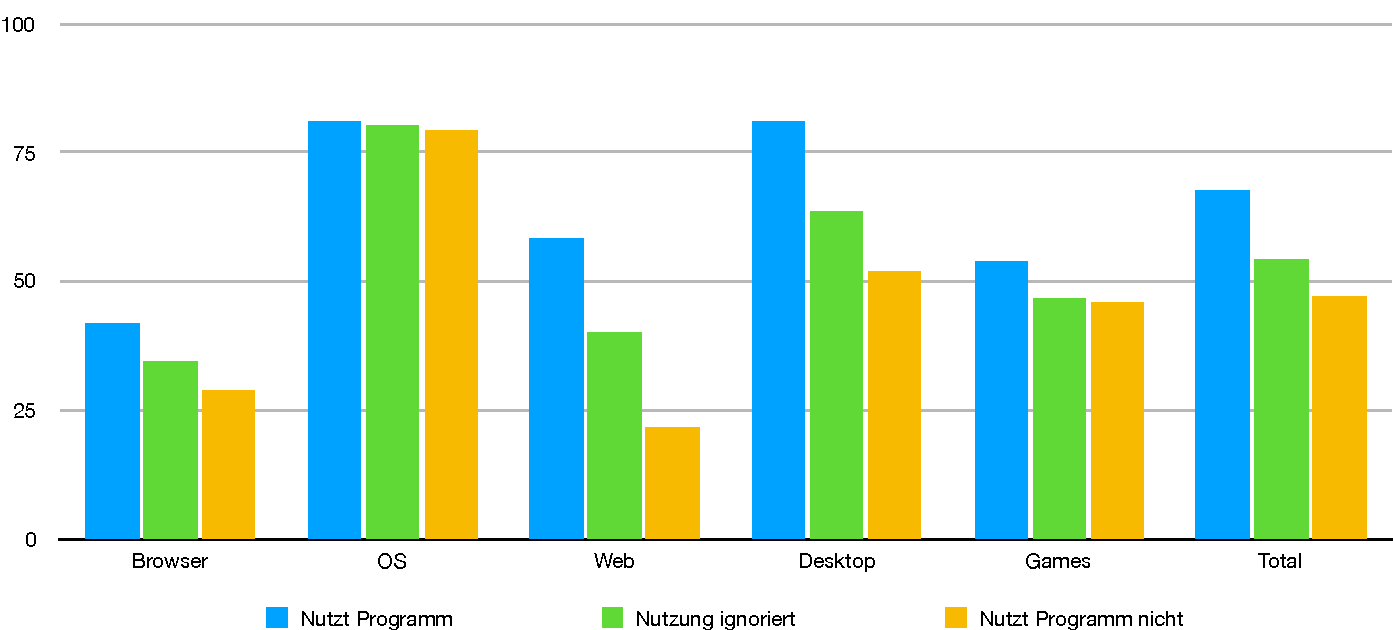
\includegraphics[width=\textwidth]{assets/results/openSourceJudging/openSourceJudging}
                \caption{Attribut Open Source  |  unbeeinflusste Nutzereinschätzung}
            \end{figure}
            Das Wissen über Open Source Software bei Endanwendern ...
            
        \subsection{Nutzung von OSS}
            Die Nutzung von OSS bei Endanwendern
        
        \subsection{Gründe für Open Source Software}
            Die Gründe für die Nutzung von Open Source Software aus Sicht der Endanwender
    
    \section{Zusammenfassung}
    
    \clearpage
    \section{Eidesstaatliche Erklärung}
        Hiermit erklären wir, dass wir die vorliegende Hausarbeit selbstständig verfasst und keine anderen als die angegebenen Hilfsmittel benutzt haben.\\
        Die Stellen der Hausarbeit, die andere Quellen im Wortlaut oder dem Sinn nach entnommen wurden, sind durch Angabe der Herkunft kenntlich gemacht. Dies gilt auch für Zeichnungen, Skizzen, bildliche Darstellungen sowie für Quellen aus dem Internet.
        
        
        \begin{figure}[H]
            \centering
            \begin{minipage}{.5\textwidth}
                \centering
                
\includegraphics[width=\textwidth]{assets/signature_tilb.png}
                Til Blechschmidt
                \label{fig:test1}
            \end{minipage}%
            \begin{minipage}{.5\textwidth}
                \centering
                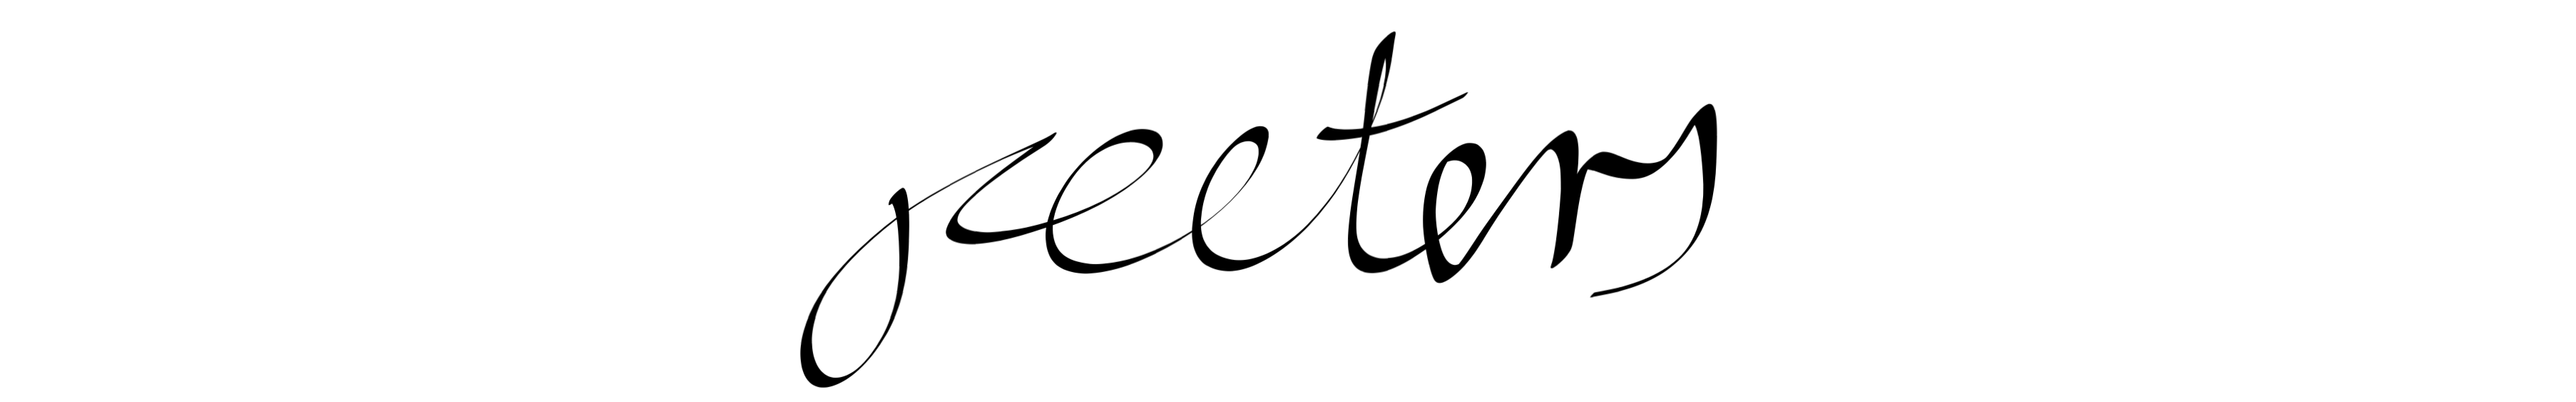
\includegraphics[width=\textwidth]{assets/signature_noahp.png}
                Noah Peeters
                \label{fig:test2}
            \end{minipage}
        \end{figure}
        \clearpage
    
    \clearpage
    \section{Appendix}
        \printglossary[type=\acronymtype]
        \printglossary
        
        \clearpage
        \nocite{*}
        \printbibliography
        
        \clearpage
        
        \subsection{Abschnitte}
            \begin{tabular}{rl}
              Abschnitt & Autor \\
              \hline
              Bla & N. Peeters\\
              Bla & T. Blechschmidt
            \end{tabular}
        
        \subsection{Umfrage}
            \paragraph{Ergebnisse}
                Die Ergebnisse der Umfrage liegen als CSV-Datei bei und sind auch in dieses PDF eingebunden: \attachfile{assets/Open Source.csv}
            \paragraph{Fragebogen}
                Auf den nächsten vier Seiten befindet sich eine PDF-Version des Fragebogens, wie er Online verbreitet wurde.
                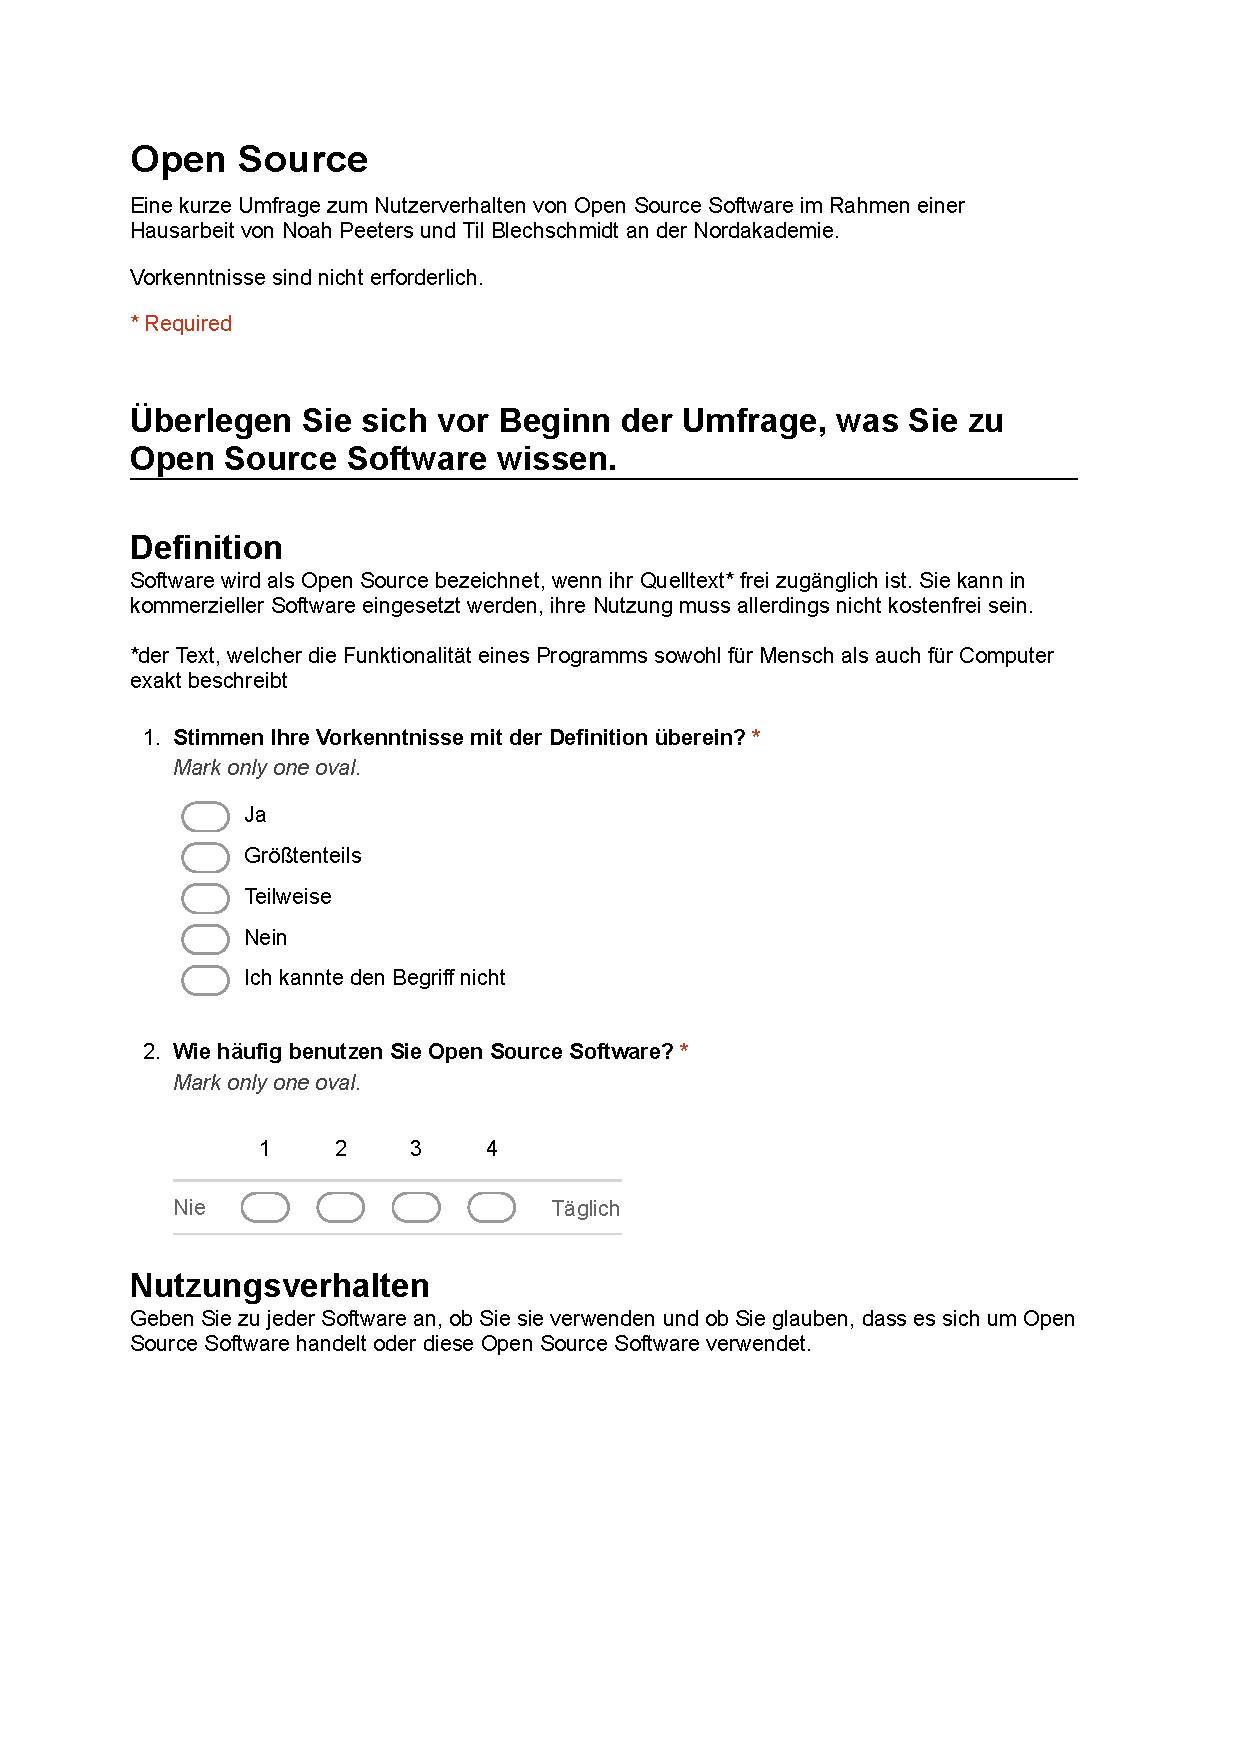
\includepdf[pages={-}]{assets/Umfrage.pdf}

\end{document}
